\section{Methodology}
    \begin{frame}
    \frametitle{Outline}
    \begin{columns}[T]
        \begin{column}{.45\textwidth}
            \tableofcontents[sections=1-3,currentsection]
        \end{column}
        \begin{column}{.45\textwidth}
            \tableofcontents[sections=4-5,currentsection]
        \end{column}
    \end{columns}
    \end{frame}
%%%%%%%%%%%%%%%%%%%%%%%%%%%%%%%%%%%%%%%%%%%%%%%%%%%%%%%%%%%%%%%%%%%%
    \subsection{Dust}
    \begin{frame}{\subsecname}
    \begin{itemize}
        \item Novel mid-fidelity aerodynamic solver based on: 
        \begin{itemize}
            \item Vortex Particle Method (VPM) $\xrightarrow{}$ Wake modeling
            \item Lifting Line Elements $\xrightarrow{}$ Solid Boundaries
        \end{itemize} 
    \end{itemize}
    \begin{figure} [H]  
	\centering
	\subfloat
	{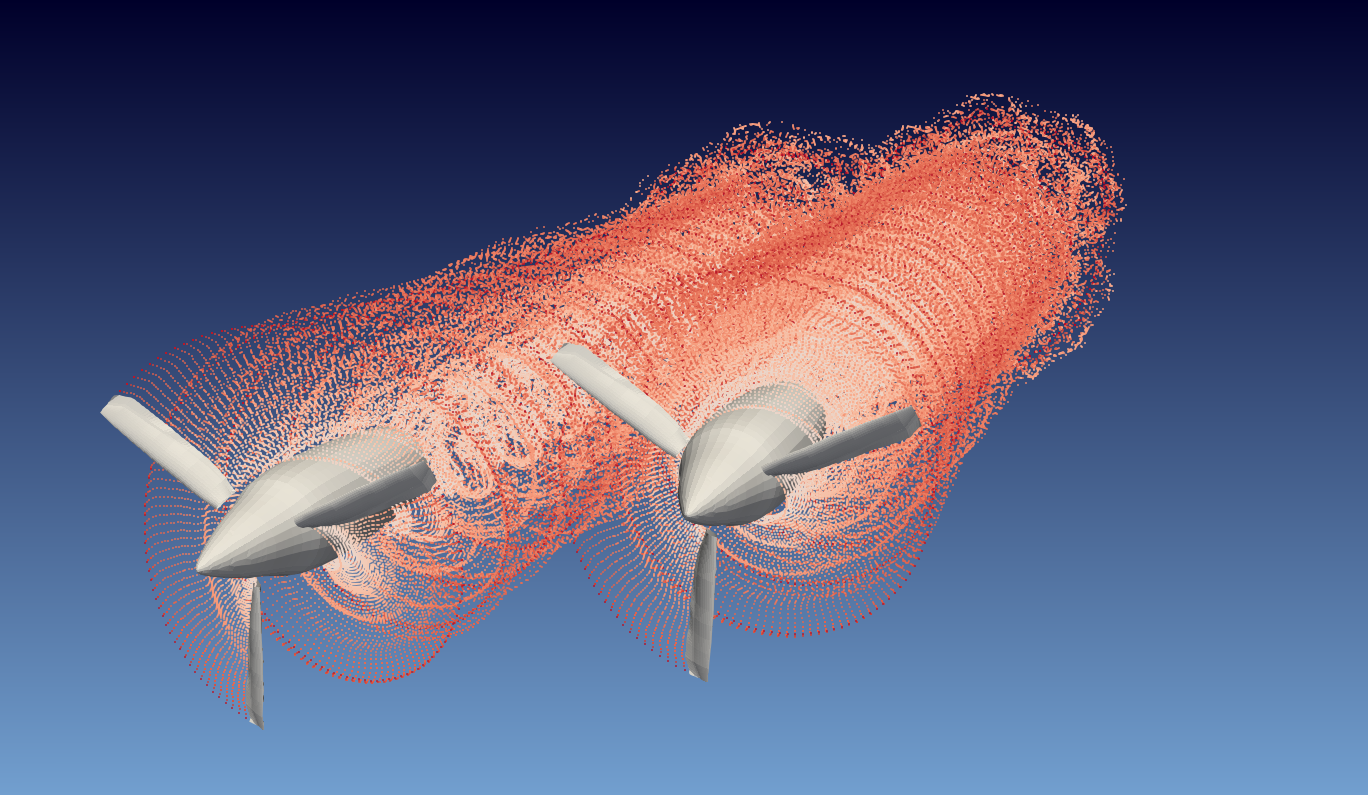
\includegraphics[scale=0.11]{Photos/2_rotors_dust_wake.eps}
  }
  \quad
	\subfloat
	{\includegraphics[scale=0.11]{Photos/2_rotors_dust__wake_side.eps}
  }
  \caption{DUST's wake visualization ($L_x$=0.1m, $L_y$=0.31m)}
\end{figure} 
    \end{frame}


\subsection{SU2 (CAA)}
\begin{frame}{\subsecname}
    \begin{itemize}
        \item FWH numeric approach
        \item Surface flow files (DUST outputs)
        \item Dummy mesh
        \item Acoustic Configuration
        \item 36 Observers, located at R = 2m:
    \end{itemize}

\begin{figure}
\subfloat [2 rotors]
	{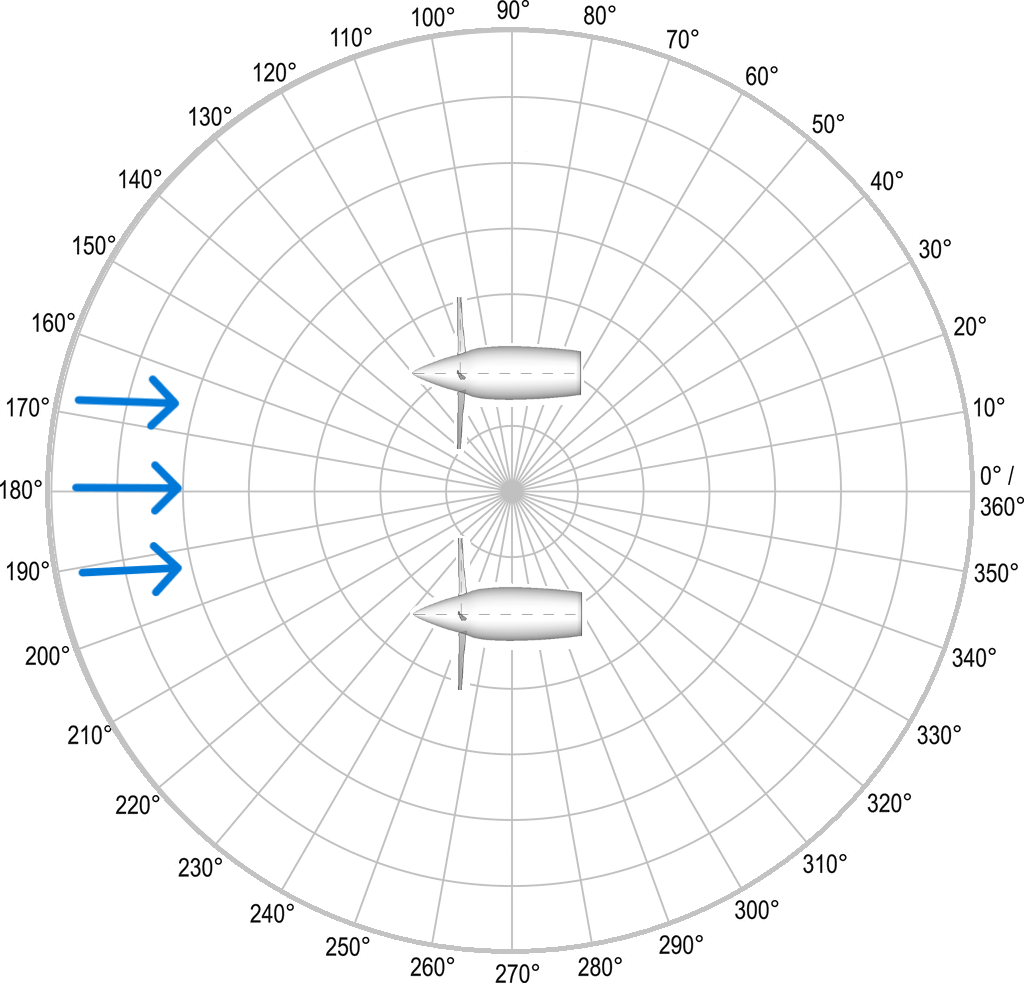
\includegraphics[scale=0.18]{Photos/observers_2rotors.png}
  }
  \quad
	\subfloat [1 rotor]
	{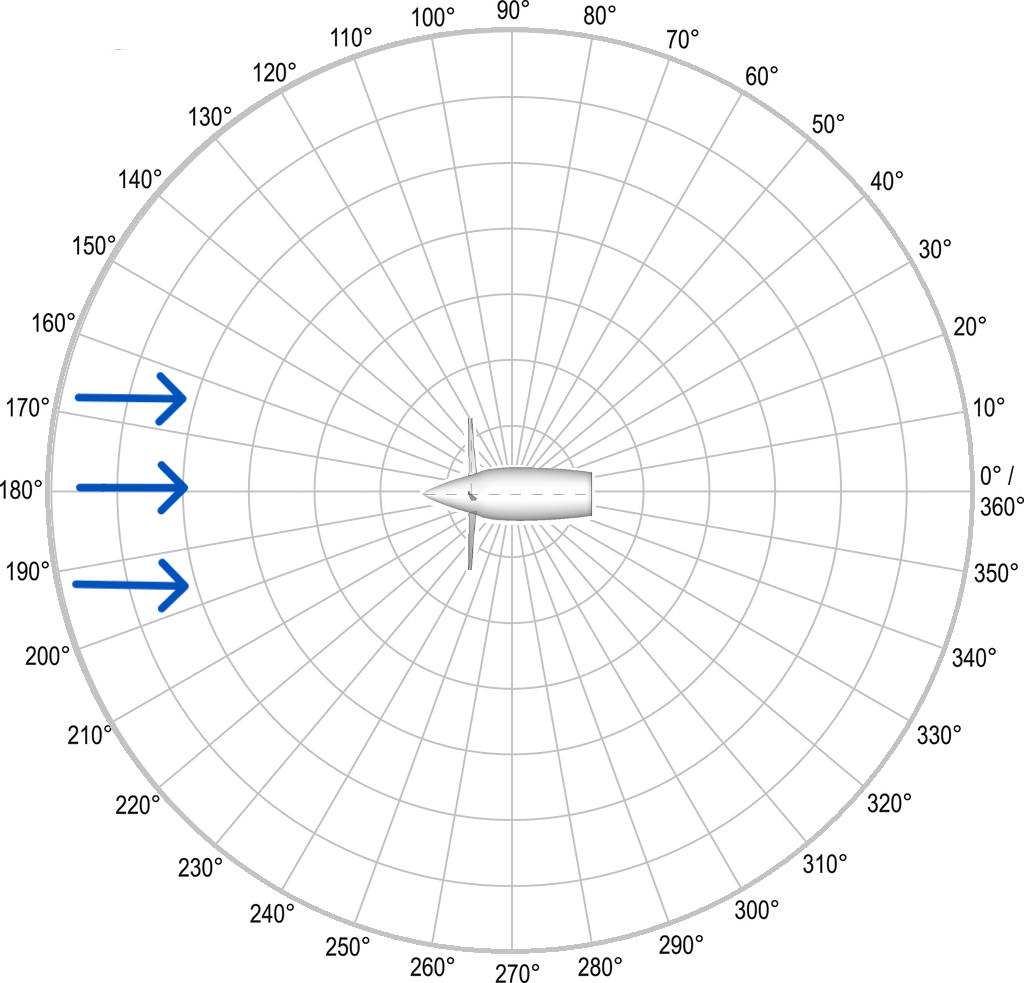
\includegraphics[scale=0.18]{Photos/observers_1rotor.png}
  }
\end{figure}

\end{frame}    


